\documentclass[12pt,a4paper]{article}
\usepackage{amsmath,amsxtra,amsthm,amssymb,makeidx,graphics,graphicx}
\begin{document}

\title{Tutorial on Topological Data Analysis}
\author{Kunlin}
\maketitle

\tableofcontents

\begin{abstract}
    This is for the first tutorial of topological data analysis. 
\end{abstract}

\section{Tutorial on \LaTeX}

This is a \textbf{bold text}. \\
This is a \underline{underlined text}. \\
This is a \textit{italic text}. 

This could  also be \underline{\textbf{\textit{combined}}}.

If you don't want to choose manually, you could use \emph{emphsize}. 

\textit{\emph{emphsize} under italic text}. 
\textbf{\emph{emphasize} under bold text}. 

\begin{figure}[h]
    \centering
    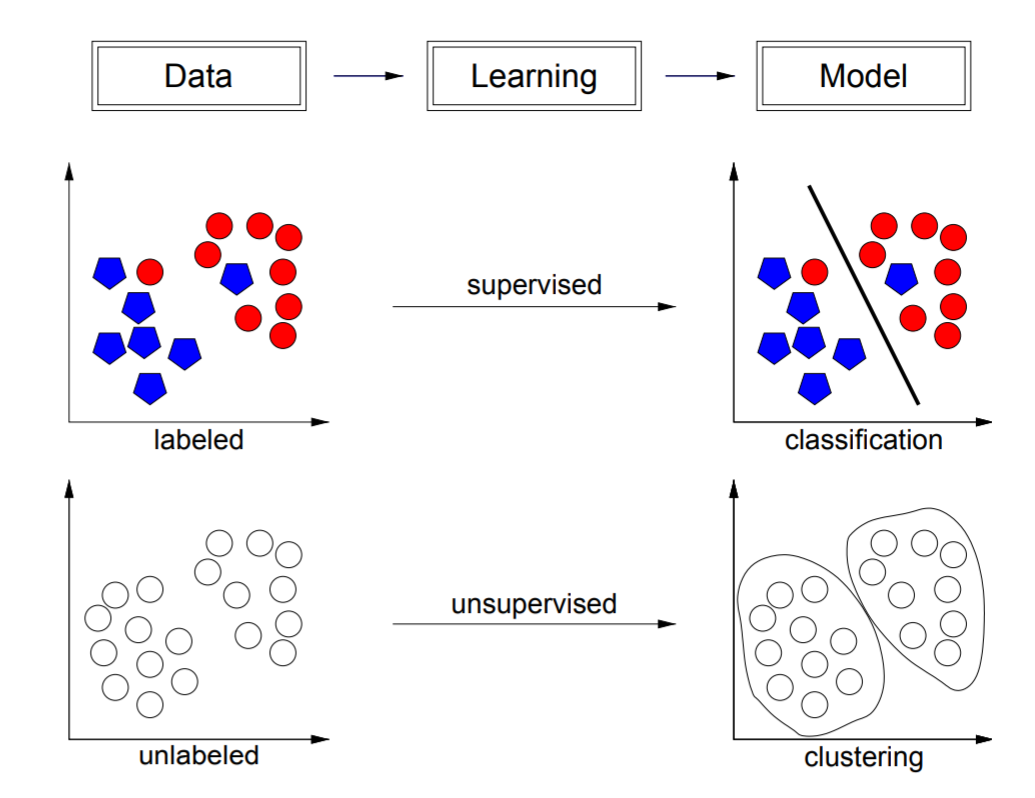
\includegraphics[width=0.8\textwidth]{img/ml.png}
    \caption{The introduction of xxx}
    \label{fig:ml}
\end{figure}

Take a look at the Figure \ref{fig:ml} . 

\begin{itemize}
    \item List one
    \item List two
\end{itemize}

\begin{enumerate}
    \item Number one
    \item Number two
\end{enumerate}

Metric: (i) $d(x,y) \geq 0$ for all $x,\,y \in X$.

\begin{equation}
    d(x,y) = 
    \begin{cases}
        0000000&\text{if $x=y$},\\
        1&\text{if $x\neq y$},
    \end{cases}
\end{equation}

\section{Metric Space}
Definition: Let $X$ be a set and $d:X^{2}\rightarrow{\mathbb R}$ a function with the follow properties:

(i) $d(x,y) \geq 0$ for all $x,\,y\in X$.

(ii) $d(x,y)=0$ if only if $x=y$. 

(iii) $d(x,y)=d(y,x)$ for all $x, \,y \in X$. 

(iv) $d(x,y)+d(y,z) \geq d(x,z)$ for all $x,\,y,\,z\in X$. (This is called the \emph{triangle inequality}).

Then we say that $d$ is a \emph{metric} on $X$ and that $(X,d)$ is a \emph{metric space}. 

Take away:

`(i) Distances are always positive. 

(ii) Two points are zero distance part if and only if they are the same point.

(iii) The distance form $A$ to $B$ is the same as the distance from $B$ to $A$. 

(iv) The distance form $A$ to $B$ via $C$ is at least as great as the distance from $A$ to $B$ directly. '
    
\end{document}